\documentclass{article}
\usepackage[paperwidth=175mm,paperheight=67mm,margin=0mm]{geometry}
\usepackage[T1]{fontenc}
\usepackage{lmodern}
\usepackage{amsmath}
\usepackage{graphicx}
\usepackage{tikz}
\usetikzlibrary{arrows.meta,backgrounds,calc}
\pagestyle{empty}
\setlength{\parindent}{0pt}
\setlength{\topskip}{0pt}

\definecolor{navy}{HTML}{1D3552}
\definecolor{ink}{HTML}{243749}
\definecolor{slate}{HTML}{526677}
\definecolor{linegray}{HTML}{A4B0BC}
\definecolor{pale}{HTML}{F1F4F7}
\definecolor{palenavy}{HTML}{E8EFF6}
\definecolor{gold}{HTML}{8E5D21}
\definecolor{palegold}{HTML}{FAF0E0}
\definecolor{panelwash}{HTML}{F8FAFD}
\definecolor{panelrule}{HTML}{8192A5}
\definecolor{blueedge}{HTML}{4977A8}
\definecolor{bluewash}{HTML}{EAF2FD}
\definecolor{tealedge}{HTML}{408278}
\definecolor{tealwash}{HTML}{E9F6F2}
\definecolor{violetedge}{HTML}{7657A3}
\definecolor{violetwash}{HTML}{F1EDFA}
\definecolor{ochreedge}{HTML}{A77838}
\definecolor{ochrewash}{HTML}{FAF0DF}

\tikzset{
  card/.style={draw=linegray,fill=pale,rounded corners=1.1mm,line width=.48pt},
  cool/.style={card,draw=navy,fill=palenavy},
  warm/.style={card,draw=gold,fill=palegold},
  labeltext/.style={align=center,text=ink,inner sep=0pt,font=\sffamily\fontsize{8.5}{9.8}\selectfont},
  accent/.style={labeltext,text=gold},
  note/.style={labeltext,text=slate,font=\sffamily\fontsize{7.5}{9}\selectfont},
  titleline/.style={labeltext,text=navy,font=\sffamily\bfseries\fontsize{9.5}{10.6}\selectfont},
  flow/.style={draw=navy,line width=.60pt,-{Stealth[length=1.42mm,width=1.1mm]}},
  residual/.style={flow,draw=slate,dash pattern=on 2pt off 1.3pt},
  gradient/.style={flow,draw=gold,dash pattern=on 2pt off 1.3pt},
  stageframe/.style={draw=panelrule,fill=panelwash,rounded corners=1.4mm,
    line width=.58pt,dash pattern=on 2.3pt off 1.6pt},
  panelhead/.style={align=center,text=navy,inner sep=0pt,
    font=\sffamily\bfseries\fontsize{9.4}{10.8}\selectfont},
  bluecard/.style={card,draw=blueedge,fill=bluewash},
  tealcard/.style={card,draw=tealedge,fill=tealwash},
  violetcard/.style={card,draw=violetedge,fill=violetwash},
  ochrecard/.style={card,draw=ochreedge,fill=ochrewash},
  canvas/.style={x=1mm,y=1mm,baseline=0pt},
}
\newcommand{\figbounds}{\path[use as bounding box] (0,0) rectangle (174.9,66.9);}
\newcommand{\card}[5]{\draw[#1] (#2,#3) rectangle (#4,#5);}
\newcommand{\labelat}[4]{\node[#1] at (#2,#3) {#4};}
% Small vector glyphs for the operations shown in the method figures.
\newcommand{\opicon}[4]{%
  \begin{scope}[shift={(#1,#2)},draw=#3,line width=.58pt,line cap=round,line join=round]
  \csname opglyph#4\endcsname
  \end{scope}%
}
\newcommand{\opglyphgrid}{%
  \draw[rounded corners=.18mm] (-1.53,-1.53) rectangle (1.53,1.53);
  \draw (-.51,-1.53) -- (-.51,1.53) (.51,-1.53) -- (.51,1.53)
        (-1.53,-.51) -- (1.53,-.51) (-1.53,.51) -- (1.53,.51);
}
\newcommand{\opglyphtext}{%
  \draw (-1.27,-1.58) -- (1.27,-1.58) -- (1.27,.62) -- (.3,1.56) -- (-1.27,1.56) -- cycle;
  \draw (.3,1.49) -- (.3,.62) -- (1.2,.62);
  \draw (-.73,.12) -- (.71,.12) (-.73,-.45) -- (.71,-.45) (-.73,-1.01) -- (.38,-1.01);
}
\newcommand{\opglyphtokens}{%
  \foreach \x in {-1.7,-.51,.68} {
    \draw[rounded corners=.19mm] (\x,-.52) rectangle (\x+.98,.52);
  }
}
\newcommand{\opglyphlayers}{%
  \draw (-1.63,.78) -- (0,1.55) -- (1.63,.78) -- (0,.01) -- cycle;
  \draw (-1.63,.12) -- (0,-.66) -- (1.63,.12);
  \draw (-1.63,-.55) -- (0,-1.33) -- (1.63,-.55);
}
\newcommand{\opglyphtune}{%
  \draw (-1.05,-1.4) -- (-1.05,.23) (-1.05,.92) -- (-1.05,1.41)
        (0,-1.4) -- (0,-.84) (0,-.15) -- (0,1.41)
        (1.05,-1.4) -- (1.05,.04) (1.05,.73) -- (1.05,1.41);
  \draw (-1.05,.58) circle (.34mm) (0,-.5) circle (.34mm) (1.05,.38) circle (.34mm);
}
\newcommand{\opglyphchat}{%
  \draw[rounded corners=.2mm] (-1.65,1.16) -- (1.65,1.16) -- (1.65,-.73)
        -- (-.07,-.73) -- (-.91,-1.43) -- (-.91,-.73) -- (-1.65,-.73) -- cycle;
  \draw (-1,.2) -- (.94,.2) (-1,-.26) -- (.34,-.26);
}
\newcommand{\opglyphloss}{%
  \draw (-1.47,1.43) -- (-1.47,-1.38) -- (1.48,-1.38);
  \draw (-1.06,.22) -- (-.45,.22) -- (-.04,.96) -- (.56,-.32) -- (.96,.46) -- (1.49,.46);
}
\newcommand{\opglyphrepeat}{%
  \draw[-{Stealth[length=.76mm,width=.60mm]}]
        (-1.45,.11) arc[start angle=176,end angle=24,radius=1.49mm];
  \draw[-{Stealth[length=.76mm,width=.60mm]}]
        (1.45,-.11) arc[start angle=-4,end angle=-156,radius=1.49mm];
}
\newcommand{\opglyphstack}{%
  \draw[rounded corners=.20mm] (-1.35,-1.46) rectangle (1.06,.78);
  \draw (-.96,1.2) -- (1.46,1.2) -- (1.46,-1.03);
  \draw (-.82,.25) -- (.52,.25) (-.82,-.35) -- (.52,-.35) (-.82,-.93) -- (.15,-.93);
}
\newcommand{\opglyphcheck}{%
  \draw[rounded corners=.24mm] (-1.54,-1.37) rectangle (1.54,1.37);
  \draw (-.91,-.04) -- (-.32,-.57) -- (.88,.63);
}
\newcommand{\opglyphchoices}{%
  \foreach \y in {1.08,0,-1.08}{
    \draw (-1.22,\y) circle (.29mm) (-.5,\y) -- (1.38,\y);
  }
  \draw[line width=1.1pt] (-1.22,0) circle (.06mm);
}
\newcommand{\opglyphstats}{%
  \draw (-1.56,0) -- (1.56,0) (-1.56,-.64) -- (-1.56,.64)
        (1.56,-.64) -- (1.56,.64);
  \draw[line width=1.07pt] (0,0) circle (.15mm);
}


\tikzset{
  deepflow/.style={residual,draw=violetedge},
  visualslot/.style={draw=tealedge,fill=tealwash,rounded corners=.4mm,line width=.45pt},
  textslot/.style={draw=blueedge,fill=bluewash,rounded corners=.4mm,line width=.45pt},
}
\begin{document}
\noindent\begin{tikzpicture}[canvas]
\figbounds

\node[panelhead,anchor=west] at (2.5,64.1) {Held-out inference};
\labelat{note}{14.7}{57.7}{Fitness Watch};
\node[inner sep=0pt] at (14.7,44.5)
  {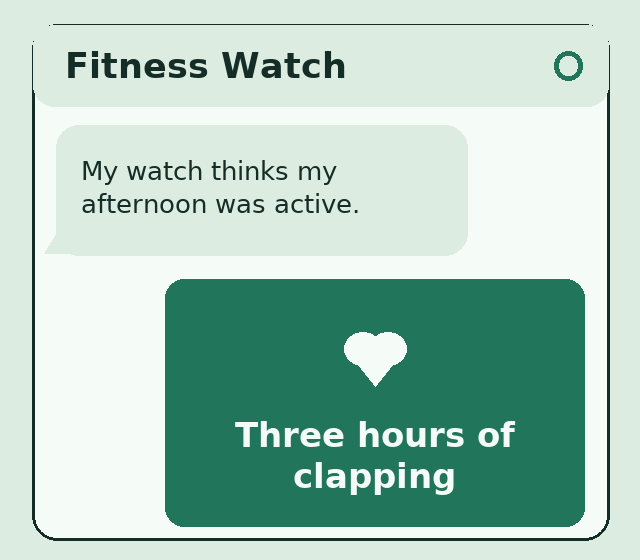
\includegraphics[height=17.5mm]{../assets/watch-original.png}};
\draw[draw=linegray,rounded corners=.55mm,line width=.48pt]
  (4.55,35.6) rectangle (24.85,53.4);

\card{bluecard}{31}{37}{59.5}{51}
\opicon{34}{46.9}{blueedge}{grid}
\labelat{labeltext}{47.3}{46.9}{\textbf{Vision encoder}}
\labelat{note}{45.25}{41.1}{24 frozen ViT blocks}
\draw[flow] (24.85,44.5) -- (31,44.5);

\card{tealcard}{66}{37}{99}{51}
\labelat{labeltext}{82.5}{46.9}{\textbf{Main patch merger}}
\opicon{71.1}{41.1}{tealedge}{tokens}
\labelat{note}{84.6}{41.1}{Visual tokens}
\draw[flow] (59.5,44.5) -- (66,44.5);

\card{card}{2.5}{16}{35.5}{29.8}
\labelat{note}{19}{26.2}{Abridged prompt}
\labelat{labeltext}{19}{20.2}{What did the\\watch count?}
\card{bluecard}{41.5}{16}{63.5}{29.8}
\labelat{labeltext}{52.5}{25.6}{\textbf{Embed text}}
\opicon{46}{20.4}{blueedge}{text}
\labelat{note}{54.2}{20.4}{Frozen}
\draw[flow] (35.5,22.9) -- (41.5,22.9);

\card{card}{70}{16}{99}{29.8}
\labelat{labeltext}{84.5}{25.6}{\textbf{Fused token stream}}
\foreach \x in {73.7,78.1,82.5}{
  \card{visualslot}{\x}{18.3}{\x+3.3}{21.7}
}
\foreach \x in {87.4,91.8}{
  \card{textslot}{\x}{18.3}{\x+3.3}{21.7}
}
\draw[flow] (82.5,37) -- (82.5,29.8);
\draw[flow] (63.5,22.9) -- (70,22.9);

% Intermediate visual features have a separate injection path.
\card{violetcard}{66}{58.4}{99}{65.8}
\labelat{labeltext}{82.5}{62.1}{\textbf{DeepStack mergers}}
\draw[deepflow] (45.25,51) -- (45.25,62.1) -- (66,62.1);
\labelat{note}{54.9}{57.5}{3 ViT taps}

\card{bluecard}{110.7}{24.1}{141.6}{48.7}
\card{bluecard}{108.6}{22.2}{139.5}{46.8}
\card{bluecard}{106.5}{20.3}{137.4}{44.9}
\labelat{labeltext}{122}{40.5}{\textbf{36 language blocks}}
\opicon{110.3}{35.5}{blueedge}{layers}
\labelat{note}{125}{35.5}{Frozen base weights}
\card{ochrecard}{111.5}{23.3}{132.5}{31}
\labelat{labeltext}{122}{27.1}{$+(\alpha/r)BA$}
\draw[flow] (99,22.9) -- (106.5,22.9);
\draw[deepflow] (99,62.1) -- (121.95,62.1) -- (121.95,48.7);
\labelat{note}{146.5}{63.0}{Added at image slots after blocks 1--3}

\card{bluecard}{146}{39.7}{172.5}{50.8}
\labelat{labeltext}{159.25}{45.25}{\textbf{Frozen LM head}}
\draw[flow] (141.6,45.25) -- (146,45.25);

\card{tealcard}{146}{16}{172.5}{32.8}
\labelat{note}{159.25}{28.4}{Structured response}
\opicon{149.1}{25.5}{tealedge}{chat}
\labelat{labeltext}{159.25}{21.7}{\textbf{Cue and relation}}
\draw[flow] (159.25,39.7) -- (159.25,32.8);

% This schematic training path is independent of the held-out example above.
\draw[draw=ochreedge,fill=ochrewash,rounded corners=.9mm,line width=.46pt]
  (2.5,1.5) rectangle (172.5,11.9);
\opicon{6.7}{6.65}{ochreedge}{tune}
\node[panelhead,anchor=west] at (10.4,6.65) {Training only};
\labelat{labeltext}{54}{8.15}{Labeled examples}
\labelat{note}{54}{3.95}{Teacher-forced forward pass}
\draw[flow,draw=ochreedge] (70,6.65) -- (75,6.65);
\opicon{78.15}{8.15}{ochreedge}{loss}
\labelat{labeltext}{94}{8.15}{\textbf{Answer-only loss}}
\labelat{note}{92.5}{3.95}{Prompt labels masked}
\draw[flow,draw=ochreedge] (107,6.65) -- (116,6.65);
\labelat{labeltext}{144.3}{8.15}{\textbf{Update LoRA} \quad $r=8,\ \alpha=16$}
\labelat{note}{144.3}{3.95}{Attention $q,k,v,o$ and MLP gate, up, down}
\draw[gradient] (122,11.9) -- (122,23.3);

\end{tikzpicture}
\end{document}
